\documentclass[conference]{IEEEtran}
\IEEEoverridecommandlockouts
% The preceding line is only needed to identify funding in the first footnote. If that is unneeded, please comment it out.
\usepackage{cite}
\usepackage{amsmath,amssymb,amsfonts}
\usepackage{algorithmic}
\usepackage{graphicx}
\usepackage{textcomp}
\usepackage{xcolor}
\usepackage{ctex}
\usepackage{fontspec}
\usepackage{listings}
\usepackage{pxfonts}
% The following code is for matlab language
\lstset{
    columns=fixed,     
    basicstyle = \tt,           % 基本样式 + 小号字体  
    %numbers=left,    % 在左侧显示行号
    frame=none,     % 不显示背景边框
    breaklines = true,                  % 代码过长则换行
    backgroundcolor=\color[RGB]{245,245,244},  % 设定背景颜色
    keywordstyle=\color[RGB]{40,40,255},         % 设定关键字颜色
    % numberstyle=\footnotesize\color{darkgray},    % 设定行号格式
    commentstyle=\it\color[RGB]{0,96,96},         % 设置代码注释的格式
    stringstyle=\rmfamily\slshape\color[RGB]{128,0,0},   % 设置字符串格式
    showstringspaces=false,   % 不显示字符串中的空格
    language=matlab,             % 设置语言
    extendedchars=false,
    %basicstyle=Consolas
    tabsize=4,
    upquote=true,
    %literate={'}{\textquotedb}1
}

\def\BibTeX{{\rm B\kern-.05em{\sc i\kern-.025em b}\kern-.08em
    T\kern-.1667em\lower.7ex\hbox{E}\kern-.125emX}}
\begin{document}

\title{傅立叶变换光谱测量技术实验报告}

\author{
    \IEEEauthorblockN{
        黄润华}
        \IEEEauthorblockA{
            \textit{Ocean University of China} \\
            \textit{email@noreply.com}
    \and
    \IEEEauthorblockN{
        杨超}
        \IEEEauthorblockA{
            \textit{Ocean University of China} \\
            \textit{email@somewhere.com}
        }
    }
}




\maketitle

\begin{abstract}
    本实验报告为傅立叶变换光谱测量技术第五次实验报告,本报告采用Python仿真动镜倾斜误差与采样间隔误差两个因素同时影响下的傅里叶变换光谱测量系统的光谱测量曲线。误差可以是随机、线性或正弦变化的。以632.8nm的HeNe激光和532nm的VAG激光为例为例。采样间隔79.1nm。本仿真以632.8nm的HeNe激光为例。
\end{abstract}

\begin{IEEEkeywords}
    Optical spectrum, python, fft
\end{IEEEkeywords}

\section{实验目的}
\begin{itemize}
    \item[1.] 思考动镜倾斜误差与采样间隔误差两个因素同时影响下的傅里叶变换光谱测量曲线形状;
    \item[2.] 学习掌握Python绘图库基础知识。 
\end{itemize} 

\section{实验原理}
\subsection{单色线的干涉方程}
理论上单色线的干涉图可以用公式(\ref{eq1})来描述
\begin{align}
    I(x) = 2cos(2\pi \sigma_0 x)    \label{eq1}
\end{align}

\subsection{采样间隔误差对干涉方程的影响}
人为进行动镜的平移过程通常掺杂着过程噪声。过程噪声的形式多种多样,常见的简单过程噪声类型为正弦噪声、随机噪声与线性噪声。然而,外部环境是一个不可预测的变量,在不同时刻的噪声类型通常是不相关且随机的,这种随机性带给光谱测量的影响是复杂性的。在操作不当的情况下,动镜移动的距离受到过程噪声的影响较大时,得到的傅立叶变换光谱测量曲线具备较低的可信度同时带来了阅读上的复杂性。

动镜移动时过程噪声带来的采样间隔误差是不可避免的,采样间隔误差的直接影响主要体现在对公式(\ref{eq1})中扫描长度$x$的影响:
\begin{align}
    I(x) = cos(2\pi\sigma_0(x + \varepsilon_s)) \label{eq9}
\end{align}

采样过程通常会选取$2^{12}$到$2^{20}$个采样点,每次采样均有可能存在一定的采样误差,采样误差经过多次迭代后对最终傅立叶光谱测量曲线带来的影响是可观且巨大的。

本次仿真模拟的采样间隔误差均为简单采样间隔误差,即代表每次采样时的误差类型为单一的正弦噪声误差、随机噪声误差或线性噪声误差。同时假设采样过程均为独立事件,前后采样过程噪声互不相干且独立。

正弦形式的采样间隔误差表达式如下:
\begin{align}
    \varepsilon_s = \frac{\lambda_0}{16}sin(2\pi\sigma_{\varepsilon}x)  \label{eq2}
\end{align}
其中波数(Wave number)数值为$\sigma_{\varepsilon} = 0.4\times10^4 m^{-1}$。

随机形式的采样间隔误差表达式可以采用均匀分布来表示:
\begin{align}
    \varepsilon_s \sim U(-\frac{\lambda_0}{5}, \frac{\lambda_0}{5})   \label{eq3}
\end{align}

线性形式的采样间隔误差表达式可以用正比例函数来表示:
\begin{align}
    \varepsilon_s(k) = k, \;\;\; k \in [0, \;79.1\times10^9 m] \label{eq4}
\end{align}

\subsection{动镜倾斜误差对干涉方程的影响}
动镜倾斜误差带来的影响从干涉图上看为在干涉图上添加一个特定的噪声:
\begin{align}
    I = cos(2\pi\sigma_0x) + \varepsilon_m \label{eq5}
\end{align}

本次仿真模拟的动镜倾斜误差均为简单动镜倾斜误差,即代表动镜倾斜误差类型为单一的正弦噪声误差、随机噪声误差或线性噪声误差。

正弦形式的动镜倾斜误差表达式如下:
\begin{align}
    \varepsilon_m = sin(2\pi\frac{\sigma_0}{16}x)  \label{eq6}
\end{align}

随机形式的动镜倾斜误差表达式可以采用均匀分布来表示:
\begin{align}
    \varepsilon_m \sim U(-1, \; 1)   \label{eq7}
\end{align}

线性形式的动镜倾斜误差表达式可以用正比例函数来表示:
\begin{align}
    \varepsilon_m(k) = k, \;\;\; k \in [0, 1] \label{eq8}
\end{align}

\subsection{综合误差对干涉方程的影响}
由式(\ref{eq9})与式(\ref{eq5})可以得到采样干涉误差与动镜倾斜误差两因素同时影响下的干涉图方程:
\begin{align}
    I = cos\left[2\pi\sigma_0(x + \varepsilon_s)\right] + \varepsilon_m    \label{eq11}
\end{align}

\section{实验内容}
仿真动镜倾斜误差因素影响下的傅里叶变换光谱测量系统的光谱测量曲线。误差可以是随机、线性或正弦变化的。以632.8nm的HeNe激光和532nm的VAG激光为例为例。采样间隔 79.1nm。

% \begin{figure*}[htbp]
% 	\centerline{
% 		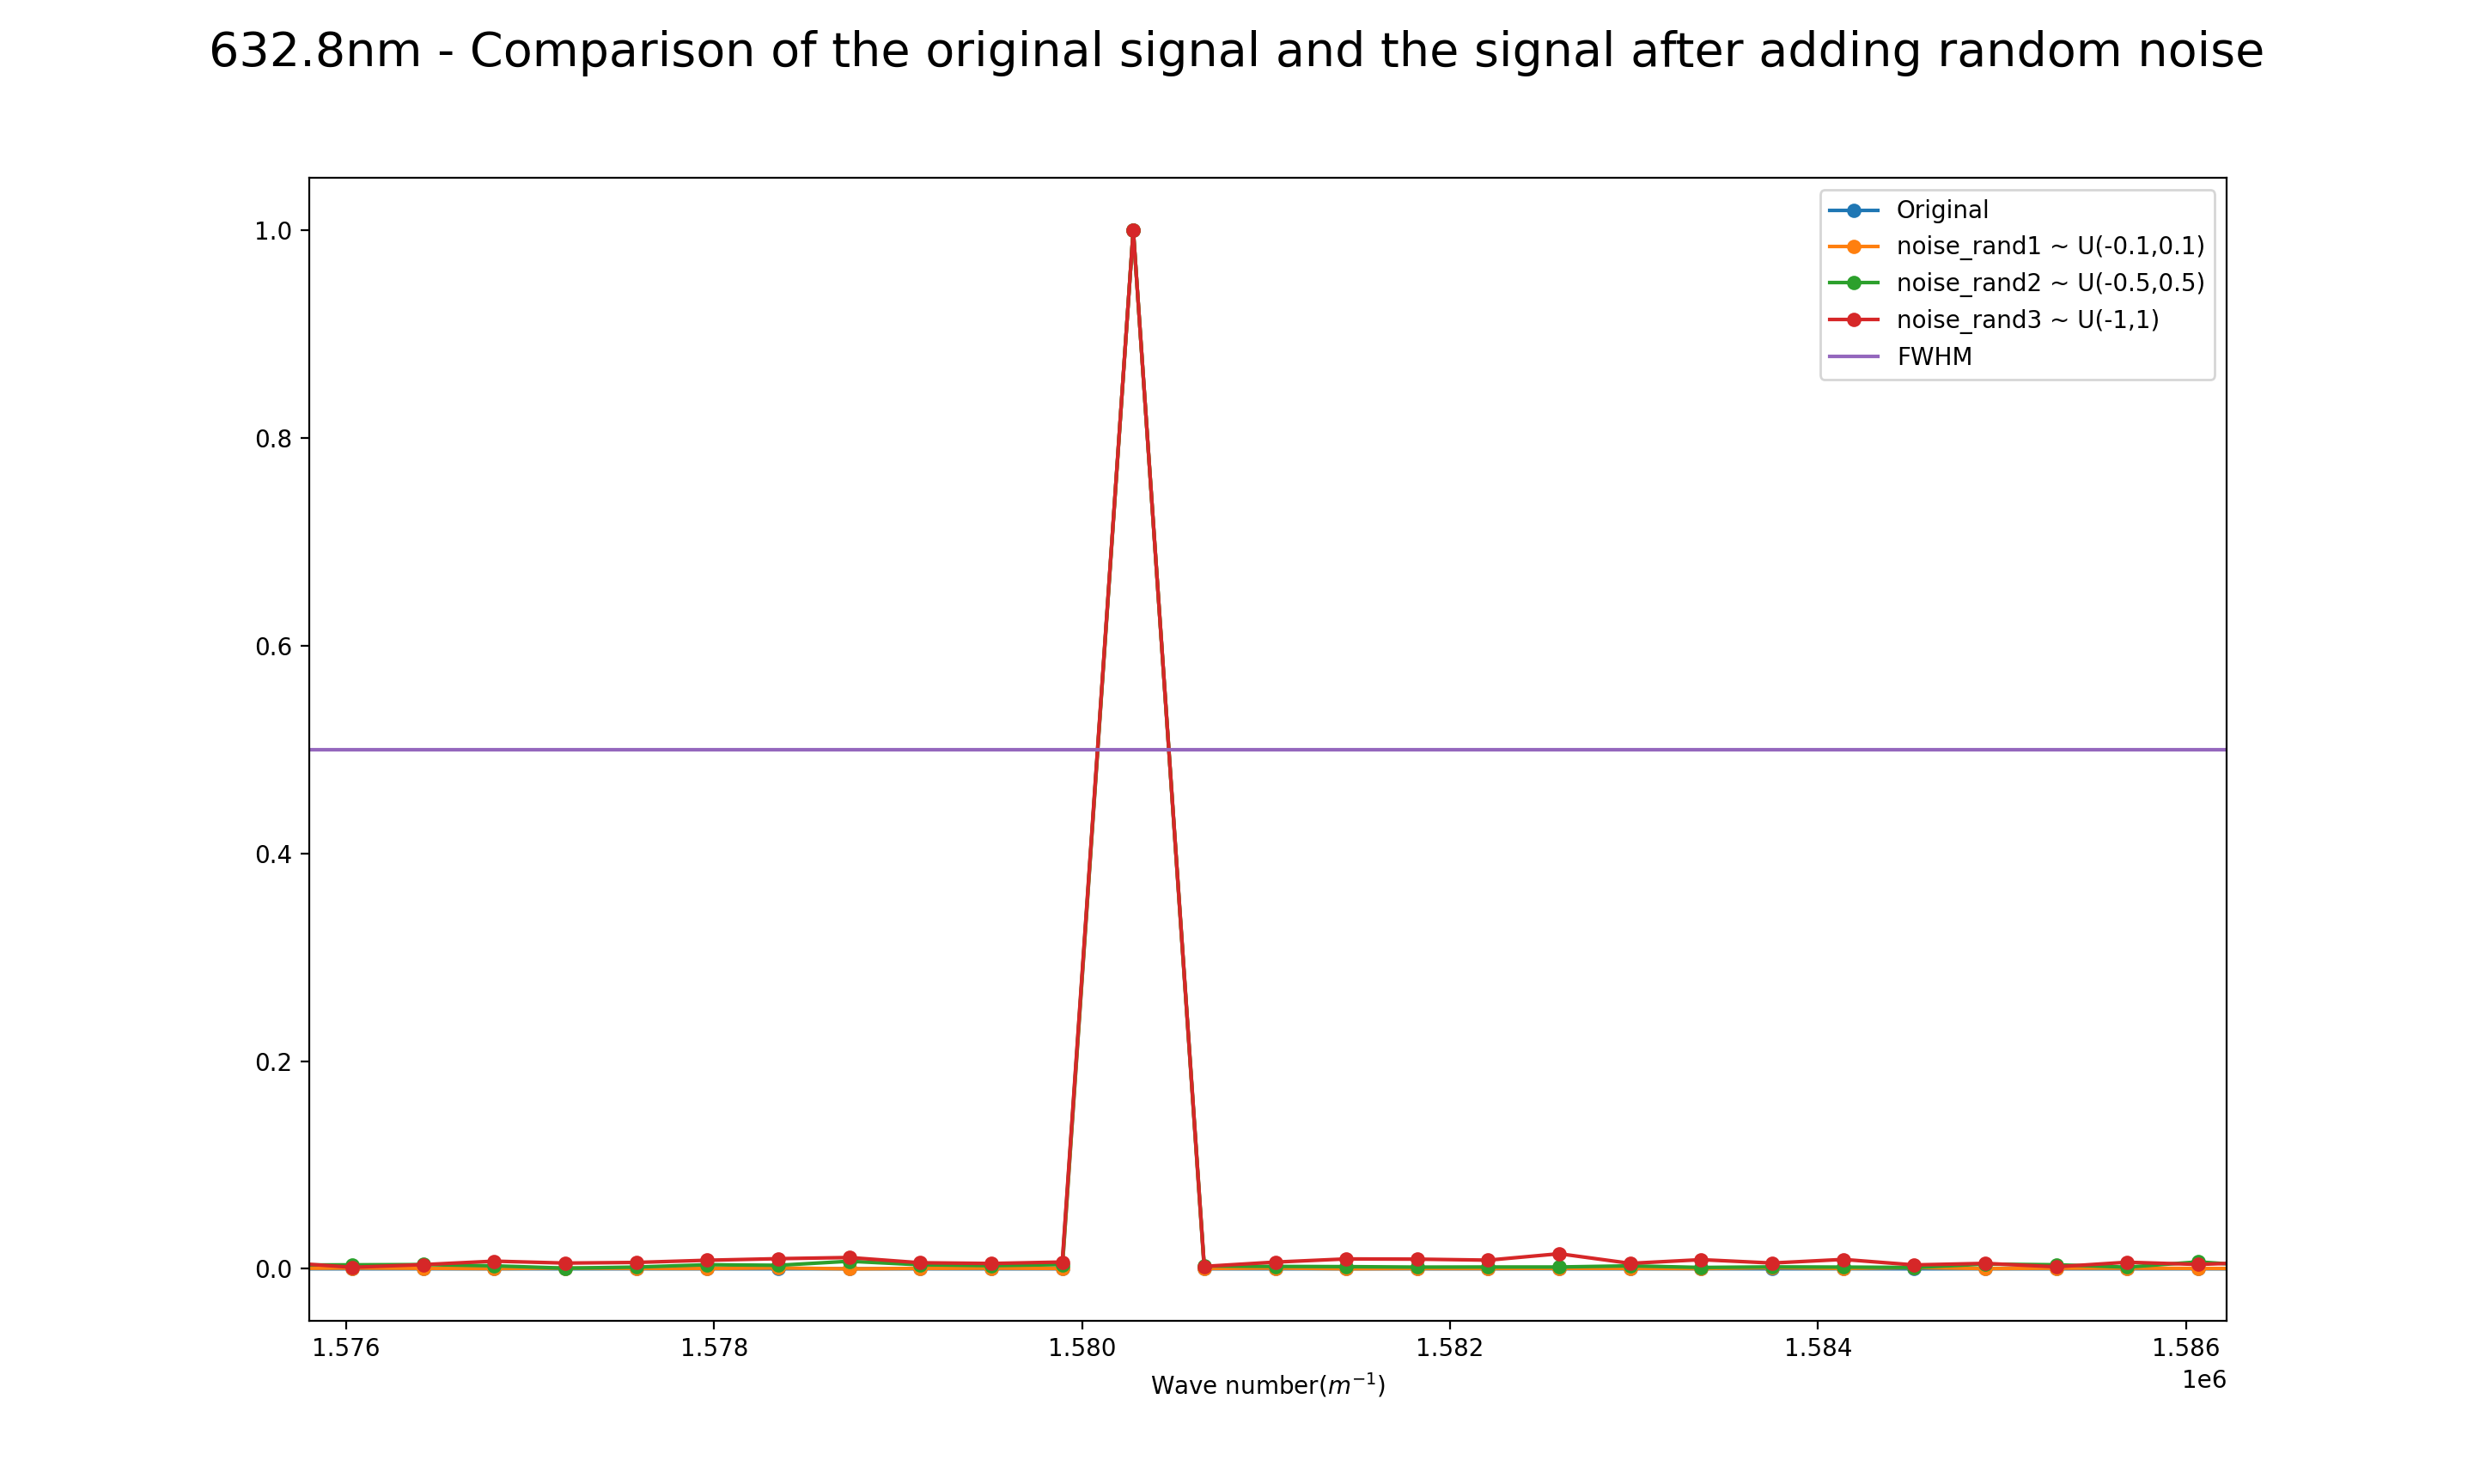
\includegraphics[width=22cm]{all.png} 	
% 	}
% 	\caption{随机噪声形式的误差对光谱曲线的影响}
% 	\label{pic7}
% \end{figure*}

\section{实验结果}
本实验报告以632.8nm的波长为例。

% \begin{figure}[htbp]
%     \centerline{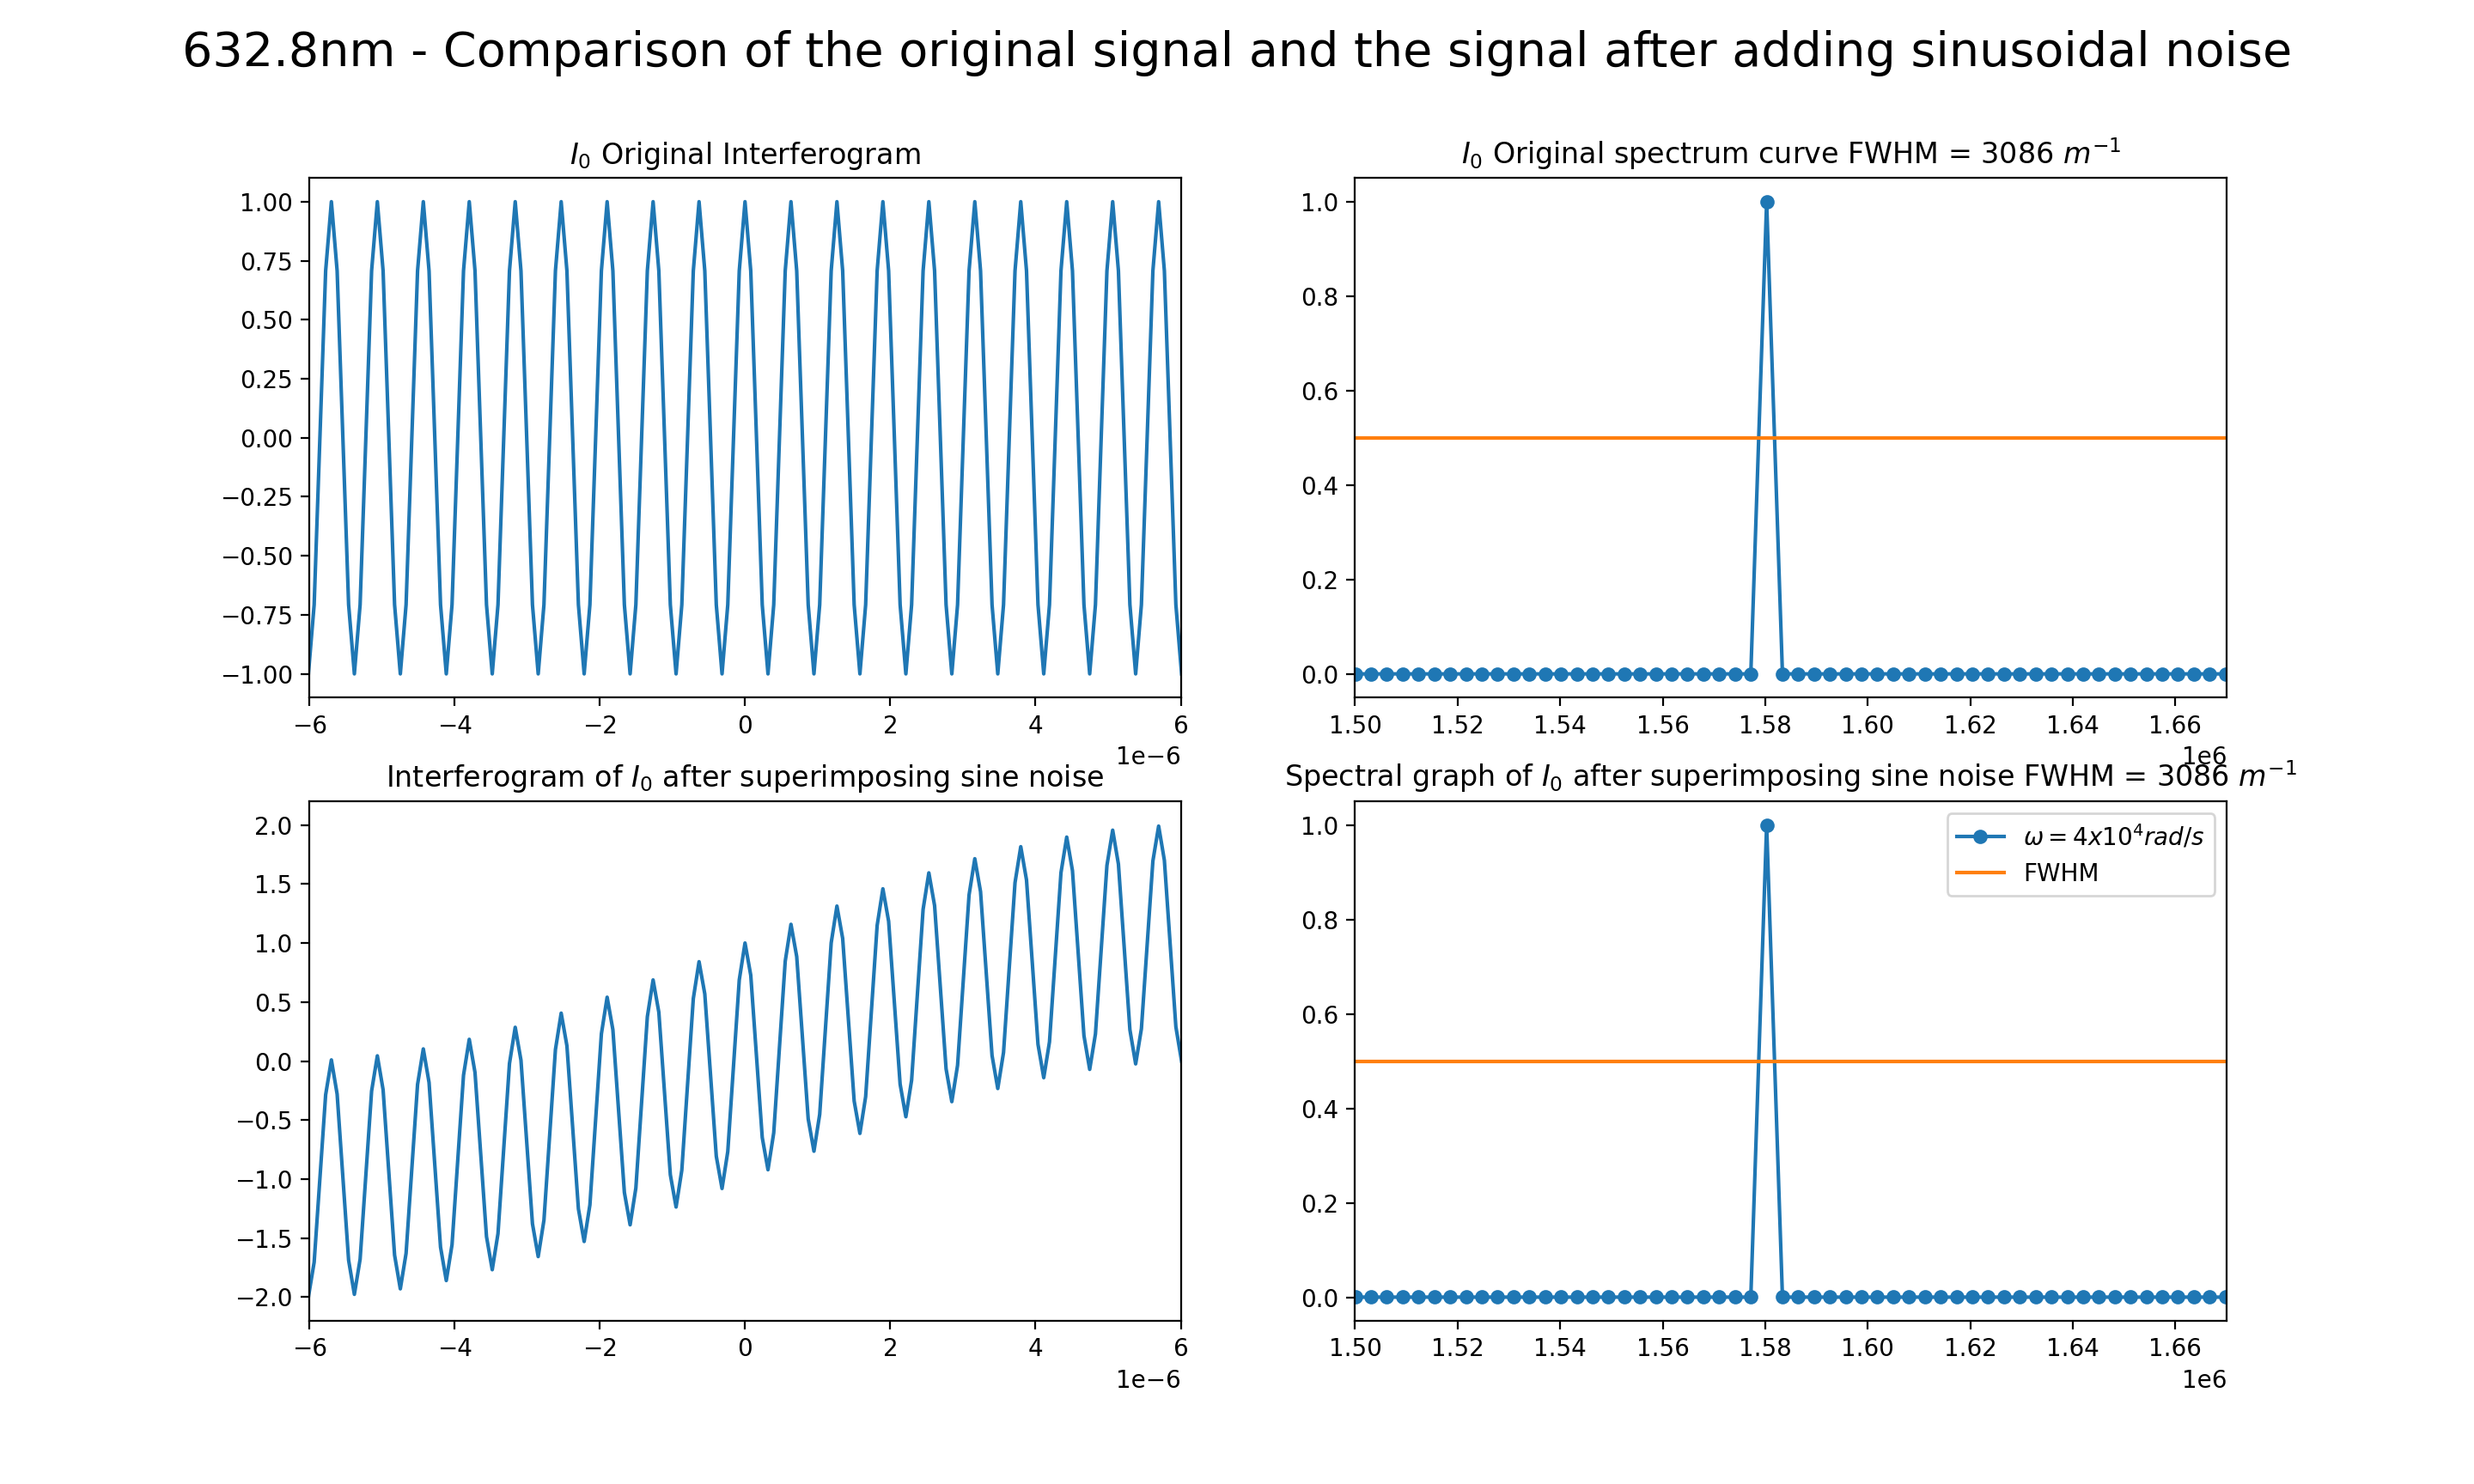
\includegraphics[width=0.5\textwidth]{6.png}}
%     \caption{叠加的正弦噪声}
%     \label{pic1}
% \end{figure}

\section{结语}
本实验完成了利用Python仿真动镜倾斜误差因素影响下的傅里叶变换光谱测量系统的光谱测量曲线。

\appendix[实验代码(以随机误差噪声为例)]
\begin{lstlisting}[language=python]
import numpy as np
import matplotlib.pyplot as plt
from scipy.fftpack import fft
from pylab import *
import random
import matplotlib.gridspec as gridspec

# 本程序模拟动镜倾斜误差影响下的傅里叶变换光谱测量系统的光谱测量曲线
# 程序具体参数如下:
#   - 采样间隔选取 79.1nm
#   - 干涉图波长选取 632.8nm
#   - 干涉图采样点数选取 2^15
#   - 本程序只叠加一种噪声----随机噪声

def GetFFT(I0, Iw0, n0):
    Y0 = 2*abs(fft(I0,n0))
    Y0_max = max(Y0);
    Y0 = Y0/Y0_max
    Y0 = Y0[:int(n0/2)]

    Yw0 = 2*abs(fft(Iw0,n0))
    Yw0_max = max(Yw0);
    Yw0 = Yw0/Yw0_max
    Yw0 = Yw0[:int(n0/2)]
    return Y0, Yw0

# 波长为632.8nm
laimda0 = 632.8*10**(-9)
# 79.1nm的采样间隔 
i = 79.1*10**(-9)
# 中心点的采样频
sigma0 = 1/laimda0
p1 = (-1)*(2**14)*79.1*10**(-9)
# 2**n个点 
p2 = (2**14-1)*79.1*10**(-9)
# 无补零 
x0 = np.arange(p1, p2, i)
n0 = n1 = 2**(int(np.log2(len(x0)))+1)
print("n0 length = %d" %n0)

I0 = np.cos(2*np.pi*sigma0*x0)

# 设置频谱图的横坐标
fs_0 = 1/i*np.arange(n0/2)/n0

#  此部分为叠加随机噪声
noise_rand = [random.uniform(-1, 1) for _ in range(len(x0))]
# noise_rand = [random.uniform(0, laimda0/5) for _ in range(len(x0))]

Iw1 = I0 + noise_rand

Y0, Yw1 = GetFFT(I0, Iw1, n0)

# 设置频谱图的横坐标
fs_1 = 1/i*np.arange(n0/2)/n0

best_Y0_average_range = 0.5*np.ones((Yw1.size, 1))

figure(1)

gs = gridspec.GridSpec(3, 6)
gs.update(wspace=0.5, hspace=0.3)

subplot(gs[0, :6])
plt.plot(x0, noise_rand)
plt.xlim(-0.00005, 0.00005)
plt.title("Waveform of random noise")

subplot(gs[1, 0:3])
s1, = plt.plot(x0, I0)
plt.legend(handles=[s1],labels=['Sample number = $2^{15}$'], loc='upper right')
plt.xlim(-6*(10**(-6)), 6*(10**(-6)))
plt.title("$I_0$ Original Interferogram")


subplot(gs[1, 3:6])
s1, = plt.plot(fs_1, Y0, marker='o', ms=5)
p1, = plt.plot(fs_0,best_Y0_average_range)
plt.legend(handles=[p1],labels=['FWHM = 385.8 $m^{-1}$'], loc='upper right')
plt.title("$I_0$ Original spectrum curve")
plt.xlim(1.5758*(10**6), 1.58622*(10**6))

subplot(gs[2, 0:3])
plt.plot(x0, Iw1)
plt.xlim(-6*(10**(-6)), 6*(10**(-6)))
plt.title("Interferogram of $I_0$ after superimposing random noise")

subplot(gs[2, 3:6])
plt.plot(fs_1, Yw1, marker='o', ms=5)
p2, = plt.plot(fs_0,best_Y0_average_range)
plt.legend(handles=[p2],labels=['FWHM = 386.9 $m^{-1}$'], loc='upper right')
plt.title("After superimposing random noise")
plt.xlim(1.5758*(10**6), 1.58622*(10**6))

plt.suptitle("632.8nm - Comparison of the original signal and the signal after adding random noise", fontsize = 20)

plt.show()

\end{lstlisting}

\end{document}
